
\documentclass[10pt,twocolumn,letterpaper]{article}
\usepackage[review]{cvpr}

\usepackage{graphicx}
\usepackage{booktabs}
\usepackage{multirow}
\usepackage{arydshln}
\usepackage{xcolor}
\usepackage{enumitem}
\usepackage{microtype}
% !TeX root = 000main.tex
% needed for compilation in TeXworks 
%\pagestyle{myheadings}

%\usepackage{amsmath,amsfonts,amssymb,rotating}
\usepackage{amssymb,amsmath,amsfonts,epsfig,mdframed,rotating,cancel,mathtools}





\usepackage{bbm}

\usepackage{comment} % To create a block comment



\newcommand{\insertfig}[3]{
\begin{figure}[tbp]\begin{center}\begin{picture}(120,90)
\put(0,-5){\includegraphics[width=12cm,height=9cm,clip=]{#1.eps}}\end{picture}\end{center}
\caption{#2}\label{#3}\end{figure}}

%
\newcommand{\inserttwofig}[4]{
\begin{figure}\begin{center}\begin{picture}(150,170)
\put(10,80){\includegraphics[with=8.5cm]{#1.ps}}
\put(10, 0){\includegraphics[with=8.5cm]{#2.ps}}
\end{picture}\end{center}
\caption{#3}\label{#4}\end{figure}}


%% Commentaires/Discussions
\newcommand{\jc}[1]{{ \color{blue} #1}}
%\newcommand{\jc}[1]{#1}

\newcommand \mqp[1]{{\color{blue}{#1}}}
%\newcommand \mqp[1]{#1}


%% Pour faire des parentheses et crochets corrects plus vite
\renewcommand{\(}{\left(}
\renewcommand{\)}{\right)}
\renewcommand{\[}{\left[}
\renewcommand{\]}{\right]}
\newcommand{\lb}{\llbracket}
%\newcommand{\rb}{\rrbracket}


% bb font symbols
%%new
\def\Q{{\mathbb Q}}
\def\C{{\mathbb C}}
\def\N{{\mathbb N}}
\def\Z{{\mathbb Z}}
\def\R{{\mathbb R}}
\def\E{{\mathbb E}}
\def\F{{\mathbb F}}
\def\P{{\mathbb P}}

%%old
\newfont{\bbb}{msbm10 scaled 500}
\newcommand{\CCC}{\mbox{\bbb C}}

\newfont{\bb}{msbm10 scaled 1100}
\newcommand{\CC}{\mbox{\bb C}}
\newcommand{\RR}{\mbox{\bb R}}
\newcommand{\ZZ}{\mbox{\bb Z}}
\newcommand{\FF}{\mbox{\bb F}}
\newcommand{\GG}{\mbox{\bb G}}
\newcommand{\LL}{\mbox{\bb L}}
\newcommand{\NN}{\mbox{\bb N}}
\newcommand{\PP}{\mbox{\bb P}}
\newcommand{\EE}{\mbox{\bb E}}
 


% Paging
\def\nn{\noindent}


% Math environnement
%\newcommand{\ds}{{\displaystyle}}
\newcommand{\D}{\displaystyle}
\newcommand{\tr}{{^{\triangle}}}

\providecommand{\ie}{{\emph{i.e.}}}


% Math Operator
\DeclareMathOperator{\ind}{1}
\def\i{\perp\!\!\!\perp} % independendent

% Vectors

\newcommand{\av}{{\bf a}}
\newcommand{\bv}{{\bf b}}
\newcommand{\cv}{{\bf c}}
\newcommand{\dv}{{\bf d}}
\newcommand{\ev}{{\bf e}}
\newcommand{\fv}{{\bf f}}
\newcommand{\gv}{{\bf g}}
\newcommand{\hv}{{\bf h}}
\newcommand{\iv}{{\bf i}}
\newcommand{\jv}{{\bf j}}
\newcommand{\kv}{{\bf k}}
\newcommand{\lv}{{\bf l}}
\newcommand{\mv}{{\bf m}}
\newcommand{\nv}{{\bf n}}
\newcommand{\ov}{{\bf o}}
\newcommand{\pv}{{\bf p}}
\newcommand{\qv}{{\bf q}}
\newcommand{\rv}{{\bf r}}
\newcommand{\sv}{{\bf s}}
\newcommand{\tv}{{\bf t}}
\newcommand{\uv}{{\bf u}}
\newcommand{\wv}{{\bf w}}
\newcommand{\vv}{{\bf v}}
\newcommand{\xv}{{\bf x}}
\newcommand{\yv}{{\bf y}}
\newcommand{\zv}{{\bf z}}
\newcommand{\zerov}{{\bf 0}}
\newcommand{\onev}{{\mathbbm 1}}
\newcommand{\Vv}{{\bf V}}   % random vector
\newcommand{\Xv}{{\bf X}}   % random vector
\newcommand{\Yv}{{\bf Y}}   % random vector
\newcommand{\Zv}{{\bf Z}}   % random vector

% Vectors with hat

\newcommand{\avh}{{\bf \hat a}}
\newcommand{\bvh}{{\bf \hat b}}
\newcommand{\cvh}{{\bf \hat c}}
\newcommand{\dvh}{{\bf \hat d}}
\newcommand{\evh}{{\bf \hat e}}
\newcommand{\fvh}{{\bf \hat f}}
\newcommand{\gvh}{{\bf \hat g}}
\newcommand{\hvh}{{\bf \hat h}}
\newcommand{\ivh}{{\bf \hat i}}
\newcommand{\jvh}{{\bf \hat j}}
\newcommand{\kvh}{{\bf \hat k}}
\newcommand{\lvh}{{\bf \hat l}}
\newcommand{\mvh}{{\bf \hat m}}
\newcommand{\nvh}{{\bf \hat n}}
\newcommand{\ovh}{{\bf \hat o}}
\newcommand{\pvh}{{\bf \hat p}}
\newcommand{\qvh}{{\bf \hat q}}
\newcommand{\rvh}{{\bf \hat r}}
\newcommand{\svh}{{\bf \hat s}}
\newcommand{\tvh}{{\bf \hat t}}
\newcommand{\uvh}{{\bf \hat u}}
\newcommand{\wvh}{{\bf \hat w}}
\newcommand{\vvh}{{\bf \hat v}}
\newcommand{\xvh}{{\bf \hat x}}
\newcommand{\yvh}{{\bf \hat y}}
\newcommand{\zvh}{{\bf \hat z}}
\newcommand{\zerovh}{{\bf \hat 0}}
\newcommand{\onevh}{{\bf \hat 1}}

% Matrices

\newcommand{\Am}{{\bf A}}
\newcommand{\Bm}{{\bf B}}
\newcommand{\Cm}{{\bf C}}
\newcommand{\Dm}{{\bf D}}
\newcommand{\Em}{{\bf E}}
\newcommand{\Fm}{{\bf F}}
\newcommand{\Gm}{{\bf G}}
\newcommand{\Hm}{{\bf H}}
\newcommand{\Id}{{\bf I}}
\newcommand{\Jm}{{\bf J}}
\newcommand{\Km}{{\bf K}}
\newcommand{\Lm}{{\bf L}}
\newcommand{\Mm}{{\bf M}}
\newcommand{\Nm}{{\bf N}}
\newcommand{\Om}{{\bf O}}
\newcommand{\Pm}{{\bf P}}
\newcommand{\Qm}{{\bf Q}}
\newcommand{\Rm}{{\bf R}}
\newcommand{\Sm}{{\bf S}}
\newcommand{\Tm}{{\bf T}}
\newcommand{\Um}{{\bf U}}
\newcommand{\Wm}{{\bf W}}
\newcommand{\Vm}{{\bf V}}
\newcommand{\Xm}{{\bf X}}
\newcommand{\Ym}{{\bf Y}}
\newcommand{\Zm}{{\bf Z}}
\newcommand{\Sigm}{{\bf \Sigma}}

% Calligraphic

\newcommand{\Ac}{{\cal A}}
\newcommand{\Bc}{{\cal B}}
\newcommand{\Cc}{{\cal C}}
\newcommand{\Dc}{{\cal D}}
\newcommand{\Ec}{{\cal E}}
\newcommand{\Fc}{{\cal F}}
\newcommand{\Gc}{{\cal G}}
\newcommand{\Hc}{{\cal H}}
\newcommand{\Ic}{{\cal I}}
\newcommand{\Jc}{{\cal J}}
\newcommand{\Kc}{{\cal K}}
\newcommand{\Lc}{{\cal L}}
\newcommand{\Mc}{{\cal M}}
\newcommand{\Nc}{{\cal N}}
\newcommand{\Oc}{{\cal O}}
\newcommand{\Pc}{{\cal P}}
\newcommand{\Qc}{{\cal Q}}
\newcommand{\Rc}{{\cal R}}
\newcommand{\Sc}{{\cal S}}
\newcommand{\Tc}{{\cal T}}
\newcommand{\Uc}{{\cal U}}
\newcommand{\Wc}{{\cal W}}
\newcommand{\Vc}{{\cal V}}
\newcommand{\Xc}{{\cal X}}
\newcommand{\Yc}{{\cal Y}}
\newcommand{\Zc}{{\cal Z}}

% Bold greek letters
% for non italic greek letters use package \usepackage{upgreek} and \boldsymbol\uptheta

\newcommand{\alphav}{\hbox{\boldmath$\alpha$}}
\newcommand{\betav}{\hbox{\boldmath$\beta$}}
\newcommand{\gammav}{\hbox{\boldmath$\gamma$}}
\newcommand{\deltav}{\hbox{\boldmath$\delta$}}
\newcommand{\etav}{\hbox{\boldmath$\eta$}}
\newcommand{\lambdav}{\hbox{\boldmath$\lambda$}}
\newcommand{\epsilonv}{\hbox{\boldmath$\epsilon$}}
\newcommand{\nuv}{\hbox{\boldmath$\nu$}}
\newcommand{\muv}{\hbox{\boldmath$\mu$}}
\newcommand{\zetav}{\hbox{\boldmath$\zeta$}}
\newcommand{\phiv}{\hbox{\boldmath$\phi$}}
\newcommand{\psiv}{\hbox{\boldmath$\psi$}}
\newcommand{\thetav}{\hbox{\boldmath$\theta$}}
\newcommand{\tauv}{\hbox{\boldmath$\tau$}}
\newcommand{\omegav}{\hbox{\boldmath$\omega$}}
\newcommand{\xiv}{\hbox{\boldmath$\xi$}}
\newcommand{\sigmav}{\hbox{\boldmath$\sigma$}}
\newcommand{\piv}{\hbox{\boldmath$\pi$}}
\newcommand{\rhov}{\hbox{\boldmath$\rho$}}

\newcommand{\Gammam}{\hbox{\boldmath$\Gamma$}}
\newcommand{\Lambdam}{\hbox{\boldmath$\Lambda$}}
\newcommand{\Deltam}{\hbox{\boldmath$\Delta$}}
\newcommand{\Sigmam}{\hbox{\boldmath$\Sigma$}}
\newcommand{\Phim}{\hbox{\boldmath$\Phi$}}
\newcommand{\Pim}{\hbox{\boldmath$\Pi$}}
\newcommand{\Psim}{\hbox{\boldmath$\Psi$}}
\newcommand{\Thetam}{\hbox{\boldmath$\Theta$}}
\newcommand{\Omegam}{\hbox{\boldmath$\Omega$}}
\newcommand{\Xim}{\hbox{\boldmath$\Xi$}}

% intercomm notation

\newcommand{\js}{(j^*)}%previous request
\renewcommand{\j}{(j)}%one arbitrary previous request
\renewcommand{\k}{(k)}%one arbitrary current request
\renewcommand{\l}{(l)}%current request
\renewcommand{\L}{(L)}%current request
\newcommand{\Ejs}{\Ec^*}%{\Ec_{j^*}}%set

\newcommand{\jm}{{(j_{m})}}% source indices of the true previous request in the set


\newcommand{\jms}{{j_{m^*}}}% indices of the true previous request in the set

%\newcommand{\Xset}{\mathcal{X}}%set of source
\newcommand{\Xl}{X_{(l)}}%arbitrary source
\newcommand{\Xone}{X_{(1)}}% first source
\newcommand{\Xk}{X_{(k)}}%requested source
\newcommand{\Xjs}{X_{(j^*)}}%previous requested source
\newcommand{\Xj}{X_{(j)}}% arbitrary previous source
\newcommand{\XJk}{X_{(J_{\k})}}% arbitrary previous source
\newcommand{\Xjone}{X_{(j_1)}}% first possible previously requested source
\newcommand{\XjM}{X_{(j_M)}}% last possible previously requested source
\newcommand{\XjMk}{X_{({j_M}_{\tiny (k)})}}% last possible previously requested source
\newcommand{\Xjm}{X_{(j_m)}}% arbitrary possible previously requested source


\newcommand{\Jsetk}{\mathcal{J}_{(k)}}%possible set of previous requested sources 
\newcommand{\Jsetkd}{\mathcal{\widetilde{J}}_{(k)}}%possible set of previous requested sources (lossy case)

\newcommand{\Mk}{M_{(k)}}%Number of possible previous requests (either  number of possible indicies or number of possible set of indices)
\newcommand{\M}{M}%Number of possible previous requests (either  number of possible indicies or number of possible set of indices)
\newcommand{\Ssetl}{\mathcal{S}_{(l)}}%possible set of previous requested sources 
\newcommand{\Rkjs}{R_{(k)|(j^*)}}%rate
\newcommand{\RkEjs}{R_{(k)|\Ec^*}}%rate
\newcommand{\Ffamk}{\mathcal{F}_{(k)}}% family of subset of possible previous requested sources
\newcommand{\sigA}{\pi}	% Ordering application
\newcommand{\Sk}{S_{(k)}}%storage

\newcommand{\Pset}{\mathscr{P}}
\newcommand{\Ppmf}{\mathcal{P}}

\newcommand{\xJxj}{_{\xv^n,\xv_{\j}^n}}  % fro the types
\newcommand{\xxj}{_{\xv^n|\xv_{\j}^n}}
\newcommand{\xxjs}{_{\xv^n|\xv_{\js}^n}}

\newcommand{\xkJxj}{_{\xv_{\k}^n,\xv_{\j}^n}}
\newcommand{\xkxj}{_{\xv_{\k}^n|\xv_{\j}^n}}
\newcommand{\xkxjs}{_{\xv_{\k}^n|\xv_{\js}^n}}


% Unknown statistics, non iid case
\newcommand{\SetET}{\boldsymbol{\hat{\theta}}^{(u_n)}}
\newcommand{\SetETR}{\boldsymbol{\widehat{\Theta}}^{(u_n)}}
\newcommand{\SetE}{\boldsymbol{\hat{\theta}}}
\newcommand{\SetER}{\boldsymbol{\widehat{\Theta}}}
\newcommand{\An}{A_{n}(\mathbf{X}^{n},\Xv_{\j}^{n})}
\newcommand{\Bn}{B_{n}(\mathbf{X}^{n},\Xv_{\j}^{n})}
\newcommand{\Vn}{V_{n}(\mathbf{X}^{n},\Xv_{\j}^{n})}
\newcommand{\Anx}{A_{n}(\mathbf{x}^{n},\xv_{\j}^{n})}
\newcommand{\Bnx}{B_{n}(\mathbf{x}^{n},\xv_{\j}^{n})}
\newcommand{\Vnx}{V_{n}(\mathbf{x}^{n},\xv_{\j}^{n})}
\newcommand{\Pt}{Q}
\newcommand{\pt}{q}

% to remove: no more used
\newcommand{\Fk}{F_{(k)}}%Number of family of subset of possible previous requested sources 
\newcommand{\Jk}{J_{(k)}}%Number of possible set of previous requested sources 



\newcommand{\tp}{\theta}
\newcommand{\Tp}{\Theta}
\newcommand{\Etp}{\mathcal{T}}
\newcommand{\tpe}{\hat{\theta}}
\newcommand{\Hs}{\overline{H}}
\newcommand{\plim}{\text{p}\text{ - }\underset{n\rightarrow \infty}{\lim\sup}~}
\newcommand{\prlim}{\text{p}\text{ -}\underset{n\rightarrow \infty}{\lim}~}

\newcommand{\sigx}{\sigma_k}
\newcommand{\sigy}{\sigma_j}
\newcommand{\cc}{\rho_{k,j}}
\newcommand{\Ckj}{\Sigma_{(k,j)}}
\newcommand{\sigkj}{\sigma_{k,j}}
\newcommand{\sigkjs}{\sigma_{k,j^{*}}}
\newcommand{\Un}{\mathbf{U}^n}
\newcommand{\un}{\mathbf{u}^n}

\newcommand{\Reqset}{\mathcal{K}} % the request set
\newcommand{\Reqvec}{\mathbf{K}} % the request vec
\newcommand{\NReq}{K} % the number of request 
\newcommand{\reqZero}{(k_0)} % the first request index
\newcommand{\reqOne}{(k_1)} % the first request index
\newcommand{\reqNReq}{(k_{\NReq})} % the Kth request index
\newcommand{\reqt}{(k_t)} % the t-th request index
\newcommand{\reqtprev}{(k_{t-1})} % the t-1-th request index

\newcommand{\G}{\mathcal{G}} % the graph
\newcommand{\V}{\mathcal{V}} % the graph
%\newcommand{\Edge}{\mathcal{E}} % the graph


% mixed symbols

\newcommand{\sinc}{{\hbox{sinc}}}
\newcommand{\diag}{{\hbox{diag}}}
\renewcommand{\det}{{\hbox{det}}}
\newcommand{\trace}{{\hbox{tr}}}
\newcommand{\sign}{{\hbox{sign}}}
\renewcommand{\arg}{{\hbox{\rm arg}}}
\newcommand{\var}{{\hbox{var}}}
\newcommand{\SINR}{\hbox{SINR}}
\newcommand{\SNR}{\hbox{SNR}}
\newcommand{\Ei}{{\rm E}_{\rm i}}
\renewcommand{\Re}{{\rm Re}}
\renewcommand{\Im}{{\rm Im}}
%\newcommand{\eqdef}{\stackrel{\Delta}{=}}
% use \triangleq instead in amsmath amssymb
\newcommand{\eqe}{\stackrel{.}{=}}
\newcommand{\<}{\left\langle}
\renewcommand{\>}{\right\rangle}
\newcommand{\smaller}{\negthickspace > \negthickspace}
\newcommand{\bit}{\mbox{ bit }}
\newcommand{\bits}{\mbox{ bits }}
\newcommand{\ifm}{\mbox{ if }}
\newcommand{\SW}{{\rm SW}}
\newcommand{\Ca}{{\rm C}}
\newcommand{\qqquad}{\qquad \quad}

\newcommand{\setN}{\{1,\,\ldots,\, N\}}
\newcommand{\setM}{\{1,\,\ldots,\, M\}}
\newcommand{\setK}{\{1,\,\ldots,\, K\}}
% math symbol

\def\<{\langle}
\def\>{\rangle}
\newcommand{\foralls}{\forall \ }
\newcommand{\indep}{\quad \begin{rotate}{90}{$\models$}\end{rotate} \quad}


\newcommand{\conv}{\ensuremath{\operatorname{conv}}}
\newcommand{\vol}{\ensuremath{\operatorname{vol}}}
\newcommand{\cut}{\ensuremath{\operatorname{cut}}}
\newcommand{\ncut}{\ensuremath{\operatorname{Ncut}}}
\newcommand{\assoc}{\ensuremath{\operatorname{assoc}}}
\newcommand{\nassoc}{\ensuremath{\operatorname{Nassoc}}}
%\newcommand{\I}{\ensuremath{\operatorname{\textbf{I}}}}

\newcommand{\I}{{\bf I}}


\newcommand{\Diag}{\ensuremath{\operatorname{Diag}}}
\newcommand{\cost}{\ensuremath{\operatorname{cost}}}

\DeclareMathOperator{\Tr}{Tr}
\DeclareMathOperator{\amin}{argmin}
%\newcommand{\sign}{\ensuremath{\operatorname{sign}}}
\newcommand{\minimize}[2]{\underset{{#1}}{\text{minimize}}\;{#2}}
\newcommand{\argmin}[1]{\underset{{#1}}{\text{argmin}}}
\newcommand{\argmax}[1]{\underset{{#1}}{\text{argmax}}}
\newcommand{\dom}{\ensuremath{\mathrm{dom}\,}}
\newcommand{\rank}{\ensuremath{\mathrm{rank}\,}}
\newcommand{\sri}{\ensuremath{\mathrm{sri}\,}}
\newcommand{\ri}{\ensuremath{\mathrm{ri}\,}}
%\newcommand{\Id}{\ensuremath{\mathrm{Id}}}
\newcommand{\prox}{\ensuremath{\operatorname{prox}}}
\newcommand{\proj}{\ensuremath{\operatorname{proj}}}
\newcommand{\fastMU}{\ensuremath{\operatorname{fastMU}}}



% ----- new macros 
\newcommand{\fid}{\ensuremath{\operatorname{fid}}}
\newcommand{\prior}{\ensuremath{\operatorname{prior}}}

\newcommand{\Jfid}{J_{\mathrm{fid}}}
\newcommand{\Jprior}{J_{\mathrm{prior}}}

\newcommand{\thetaG}{\thetav_\Gamma}
\newcommand{\thetaC}{\thetav_C}

\newcommand{\Gammatheta}{\Gamma_{\thetav_\Gamma}}
\newcommand{\Ctheta}{C_{\thetav_C}}  
\newcommand{\Phitheta}{\Phi_{\thetav_\Phi}}  
\newcommand{\Rtheta}{R_{\thetav_R}}  

\newcommand{\Ttheta}{T_{\thetav}}
\newcommand{\gphi}{g_{\phiv}}

\newcommand{\loss}{\mathcal{L}}
\newcommand{\losstraj}{\mathcal{L}_{\mathrm{traj}}}
\newcommand{\lossfinal}{\mathcal{L}_{\mathrm{final}}}
\newcommand{\losssmooth}{\mathcal{L}_{\mathrm{smooth}}}
\newcommand{\lossstep}{\mathcal{L}_{\mathrm{step}}}





% ----------

\newcommand{\fastMUmin}{\ensuremath{\operatorname{fastMUmin}}}
\newcommand{\MU}{\ensuremath{\operatorname{MU}}}
\newcommand{\kmax}{\ensuremath{K_\text{max}}}



\DeclarePairedDelimiter\ceil{\lceil}{\rceil}
\DeclarePairedDelimiter\floor{\lfloor}{\rfloor}

 		



%\renewenvironment{proof}{\textbf{Proof}}{\qed}

%%% tikz for graph 

\usepackage{tikz,tkz-tab}

\usetikzlibrary{fit,automata,positioning,calc,shapes}
\usepackage{ifthen}

\ifdefined\circlenode
\else
\newcommand{\circlenode}[3]{
	\node [draw, circle, inner sep=2pt, #1] (#2) {#3};
}
\fi
\ifdefined\sqnode
\else
\newcommand{\sqnode}[3]{
	\node [draw, rectangle, inner sep=2pt, #1] (#2) {#3};
}
\fi



%%% index

\newcommand{\iopt}{\overline{i}}
\newcommand{\jopt}{\overline{j}}
\newcommand{\topt}{\overline{t}}
%\usepackage{amsthm} % Load theorem package

 

%%%%% color definition 
\definecolor{darkgreen}{rgb}{0.1,0.5,0}
\definecolor{Midnightblue}{rgb}{.2,.2,.7}
\definecolor{mypink3}{cmyk}{0, 0.7808, 0.4429, 0.1412}

\def\blue#1{\textcolor{Midnightblue}{#1}}

\def\bblue#1{\textbf{\textcolor{Midnightblue}{#1}}}

\definecolor{amber}{rgb}{1.0, 0.49, 0.0}

\def\oran#1{\textcolor{amber}{#1}}

\def\redm#1{\textcolor{mypink3}{#1}}

\def\boran#1{\textbf{\textcolor{amber}{#1}}}
\def\green#1{\textcolor{darkgreen}{#1}}


% remove/comment the sentence 

\newcommand \remove[1]{ }

 




 


\newcommand{\TODO}[1]{\textbf{\color{red}[TODO: #1]}}

\definecolor{cvprblue}{rgb}{0.21,0.49,0.74}
\usepackage[pagebackref,breaklinks,colorlinks,allcolors=cvprblue]{hyperref}

\def\confName{CVPR}
\def\confYear{2027}

\title{GALA: Gallery-Level Alignment for Real-Life BCI Deployment\\on Unseen Subjects}

\author{Anonymous CVPR submission}

\begin{document}
\maketitle

%=====================================================================
\begin{abstract}
Neural decoding of visual experience from electroencephalography (EEG) has achieved strong performance in intra-subject settings, but current methods fail to generalize across individuals: on the standard 200-way benchmark THINGS-EEG-2, top-1 accuracy drops from above 80\% within subjects to about 32\% for an unseen subject. In a practical brain-computer interface (BCI), however, the possible outcomes that we are trying to decode are known in advance, and constitute a predefined list of candidates, the gallery. Adapting a pre-trained encoder to new subjects and new sessions traditionally requires labeled data, which is often prohibitively expensive to obtain. We argue instead for gallery-level alignment, in which the unlabeled EEG signal of the user, taken as a whole, is gradually aligned to the known gallery of outcomes during the usual deployment of the BCI, with no need for collecting any labels. We formalize this setting as \emph{label-free transductive subject calibration}, and propose an evaluation protocol with regimes closer to the conditions of a deployed BCI. Within this protocol, we introduce \textbf{GALA} (\textbf{GA}llery-\textbf{L}evel \textbf{A}lignment), a label-free calibration method which registers the unlabeled EEG embeddings onto the gallery through shrinkage whitening, hubness correction and iterated Sinkhorn--Procrustes alignment. Without any labeled data from the new subject, GALA raises cross-subject top-1 accuracy on THINGS-EEG-2 from 32.2\% to 81.8\%. 
\end{abstract}

%=====================================================================
\section{Introduction}
\label{sec:intro}

Decoding visual perception from brain activity is a central goal of neuroscience~\cite{kamitani2005decoding,carlson2013representational,grootswagers2017decoding}, with applications ranging from the study of visual representations~\cite{cichy2014resolving,contini2017decoding} to assistive brain-computer interfaces~\cite{lawhern2018eegnet,gao2021interface}. EEG is especially attractive for this problem because it is non-invasive, has high temporal resolution, and is relatively inexpensive. In the now-standard \emph{EEG-to-image retrieval} setting~\cite{spampinato2017deep,gifford2022things,grootswagers2022things}, EEG signals and images are represented in a joint embedding space, and retrieval selects, for a given EEG signal, the closest image from a candidate set. Following progress in fMRI-to-image decoding~\cite{takagi2023highres,ozcelik2023natural,scotti2023mindeye,scotti2024mindeye2}, recent work aligns EEG embeddings with features from large pre-trained vision models through contrastive learning~\cite{song2024nice,li2024atm,wu2025ubp,zhang2025neurobridge,du2025shallow}, and now exceeds 80\% top-1 accuracy in the \emph{intra-subject} 200-way setting~\cite{du2025shallow}. In the \emph{cross-subject} setting, where the encoder must generalize to a held-out subject under the leave-one-subject-out (LOSO) protocol, accuracy remains between 20\% and 30\% for the strongest published encoders~\cite{du2025shallow,zhang2025neurobridge,cui2026score}.

\begin{figure}[t]
  \centering
  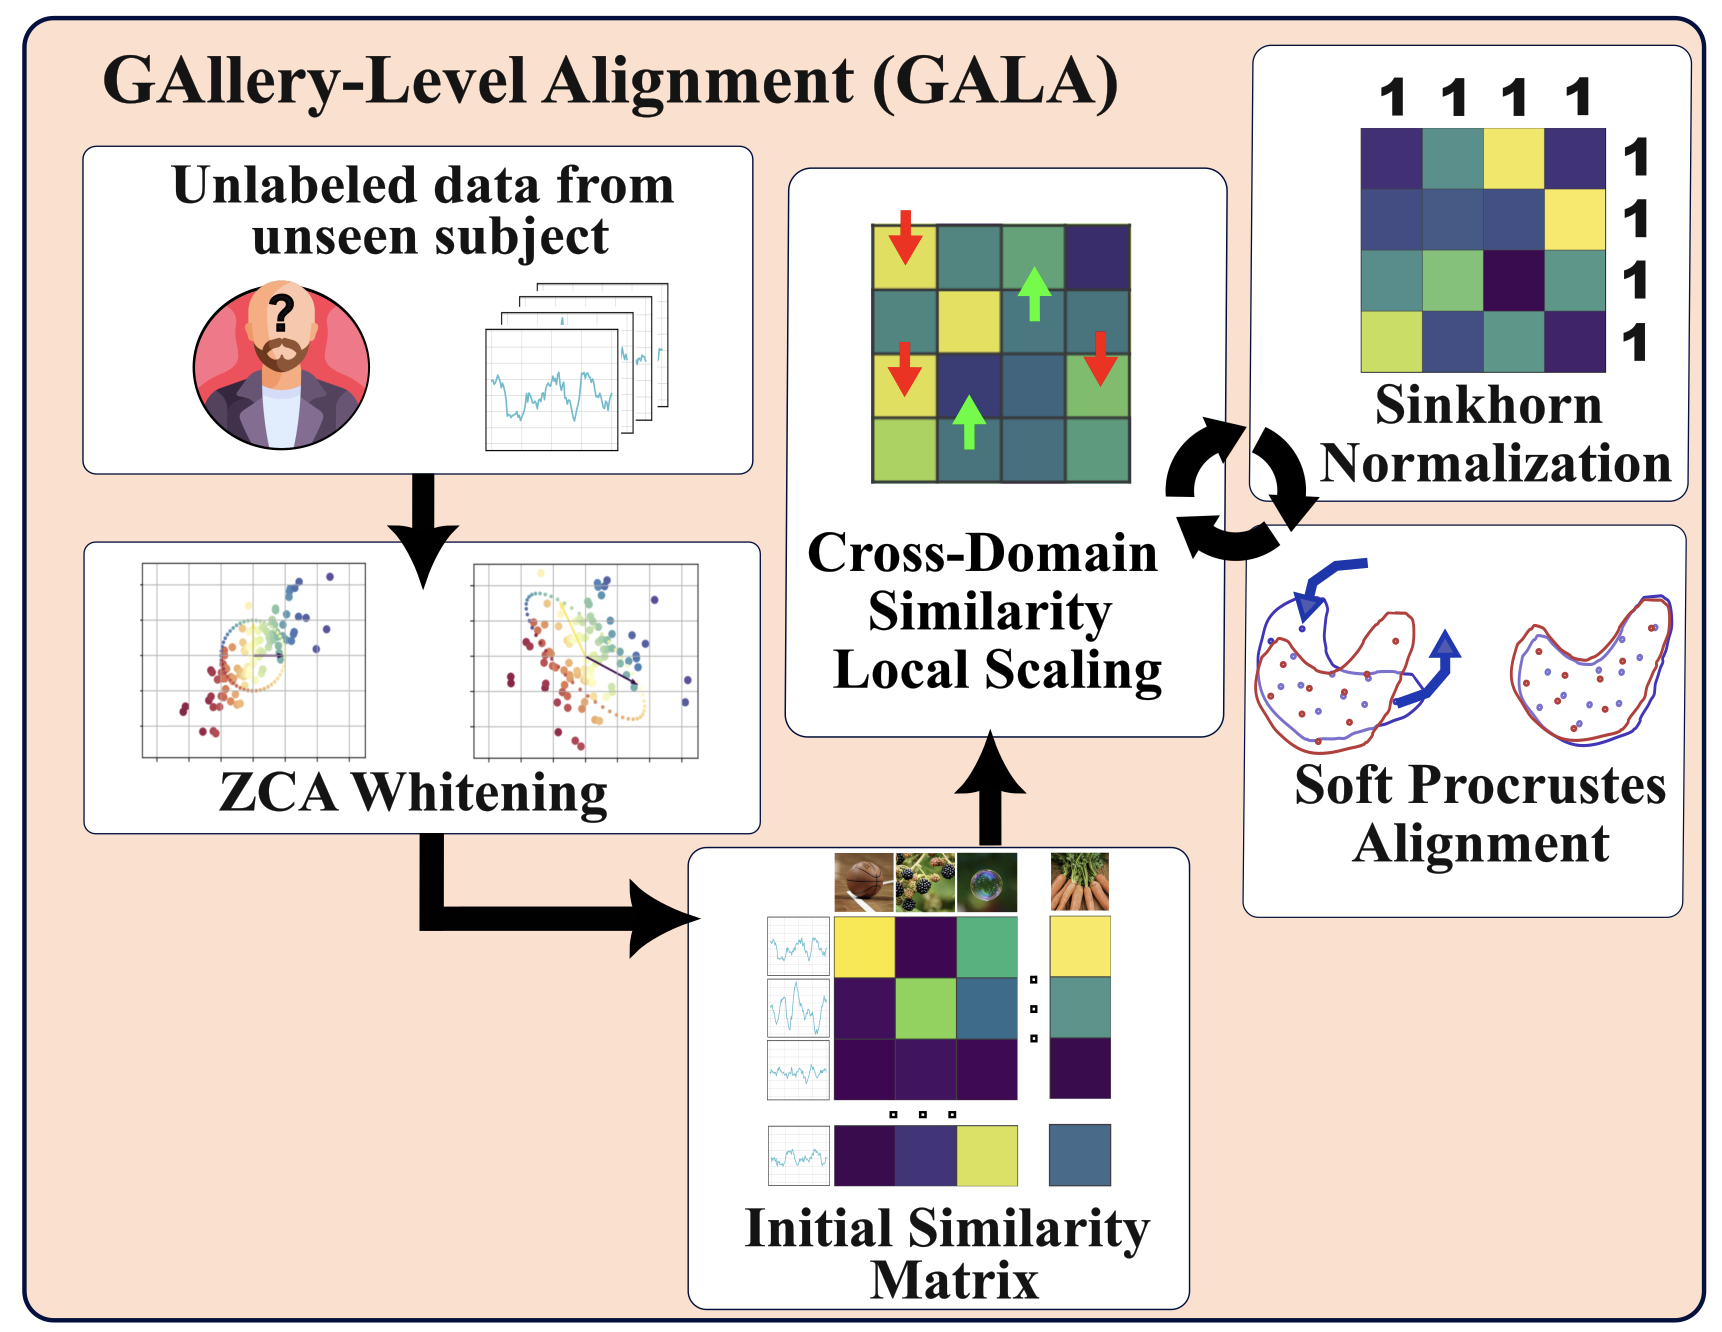
\includegraphics[width=\columnwidth]{figures/GALA.png}
  \caption{GALA. The unlabeled EEG embeddings of an unseen subject are whitened, compared with the gallery through cross-domain similarity local scaling, and registered onto it by alternating Sinkhorn normalization and soft Procrustes alignment.}
  \label{fig:pipeline}
\end{figure}

This gap is rooted in the inter-subject variability of EEG: skull geometry, cortical folding and electrode placement induce a different spatial mixing of the underlying neural sources for each individual~\cite{onton2006imaging}, and inter-subject differences in covariance structure further amplify this mismatch~\cite{blankertz2008optimizing,barachant2010riemannian,samek2013transferring,haufe2014interpretation}. How these differences produce the loss of accuracy on a new subject remains open~\cite{li2026crosssubject,lin2026identitytrap}.

In a practical brain-computer interface, the set of possible outcomes is known in advance. A user working with a mail client may want to open a folder, read an email or delete it, and an assistive interface offers a fixed menu of items. Decoding then amounts to matching the EEG signal of the user to a predefined list of candidates, the gallery, which is the retrieval setting described above. The main obstacle to deployment is the shift of the EEG signal between subjects, and between sessions of the same subject. Previous methods correct it by fine-tuning on labeled data~\cite{kneeland2025enigma}, but acquiring labeled calibration data for each new subject is often impractical, and even more so for each new session. A deployed decoder, however, knows its gallery and receives unlabeled signal from its user as soon as it is used. We therefore argue for gallery-level alignment, in which the unlabeled EEG embeddings of the user, taken together, are aligned to the known gallery without any labeled data. 

Unlike the unsupervised re-centering used in classical BCI, this alignment is performed \emph{across modalities}, onto the point cloud that the gallery forms in the embedding space. Two recent methods follow this idea~\cite{huang2026sattc,cui2026score}, but each evaluates in its own regime and with its own model selection rule, and neither states what its test-time procedure assumes about the unlabeled data, which makes their results difficult to compare. Moreover, current EEG-to-image benchmarks only measure two extremes: a zero-shot decoder that sees nothing of the new subject, and an intra-subject decoder trained on hours of labeled recordings. We propose an evaluation framework between these two extremes, closer to the conditions of a deployed BCI.

Throughout the paper, we distinguish two settings. \emph{Zero-shot} denotes the inductive cross-subject encoder evaluated without test-time adaptation, as in most prior work. \emph{Calibrated} denotes a transductive procedure that processes the unlabeled queries of the held-out subject together with the candidate image set. Our contributions are summarized as follows:
\begin{enumerate}[leftmargin=1.3em,itemsep=1pt,topsep=2pt]
  \item We formalize calibration from unlabeled target data and a known gallery, state four assumptions that existing evaluations leave implicit, and define four test regimes that, together, allow for a proper evaluation of this second category of procedures.
  \item We introduce GALA, which casts calibration as a point-cloud registration problem~\cite{besl1992method,grave2019wasserstein}: after shrinkage whitening and CSLS~\cite{conneau2018muse}, it alternates Sinkhorn correspondence estimation~\cite{cuturi2013sinkhorn} and Procrustes alignment~\cite{schonemann1966procrustes} to register the query cloud onto the gallery, with a single budget-dependent damping for short streams. On THINGS-EEG-2, GALA reaches 81.8\% top-1 across three training seeds without any labeled data from the new subject, and improves on every other label-free method for every subject.
  \item We show that the other label-free calibrations we evaluate add nothing beyond a one-to-one (Hungarian) assignment of the zero-shot scores in the standard evaluation setting, which highlights the limits of both these methods and this criterion. GALA is the only one that improves on it, by 18 points.
  \item We evaluate GALA on six encoders, on which it fixes 38\% to 73\% of the zero-shot errors, and compare this gain with the zero-shot accuracy of each encoder and with the representational similarity between its EEG and image embeddings~\cite{kriegeskorte2008rsa}.
  \item We identify the regimes in which GALA performs poorly, namely open galleries with many distractor images, and suggest options to mitigate them.
\end{enumerate}
Unlike most previous work, we report every cross-subject number without leakage from the test subject: checkpoints are selected on held-out training concepts, and calibration hyper-parameters on the other LOSO folds. We encourage other authors to report their results under the same protocol.
The full training and evaluation code, as well as the configuration files for every reported run and the trained checkpoints, will be released publicly.

%=====================================================================
\begin{figure*}[t]
  \centering
  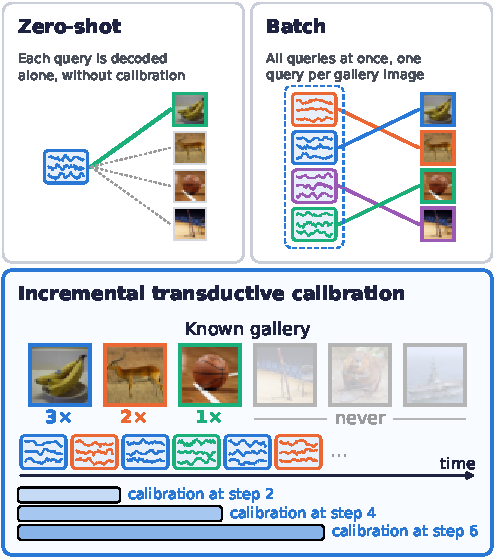
\includegraphics[width=\textwidth]{figures/protocol.pdf}
  \caption{The four evaluation regimes. R0: each query is decoded alone against the gallery. R1: the 200 test queries are calibrated together, and each gallery image is queried exactly once. R2: queries from a menu of $K$ images arrive one at a time, possibly repeated, and the calibration is re-fitted on the growing buffer. R3: $D$ distractor images that are never queried are added to the gallery. EEG traces are illustrative; images are from the THINGS-EEG-2 test set.}
  \label{fig:protocol}
\end{figure*}

\section{Related Work}
\label{sec:related}

\paragraph{EEG-to-image decoding.}
Visual neural decoding has progressed from early supervised, subject-specific classifiers on labeled EEG-image pairs~\cite{spampinato2017deep,du2023bravl} to a zero-shot retrieval paradigm enabled by large-scale serial visual presentation benchmarks~\cite{gifford2022things,grootswagers2022things}.
NICE~\cite{song2024nice} established the contrastive alignment framework, using an InfoNCE~\cite{oord2019cpc} objective to align TSConv EEG embeddings with frozen CLIP~\cite{radford2021clip} image features.
UBP~\cite{wu2025ubp} dynamically blurs image targets proportional to stimulus uncertainty, while NeuroBridge~\cite{zhang2025neurobridge} introduced principled image augmentation for better bidirectional alignment.
ENIGMA~\cite{kneeland2025enigma} adapts to new subjects in a few-shot setting through subject-specific latent layers coupled with a compact bottleneck.
Shallow Alignment~\cite{du2025shallow} showed that intermediate-layer features of large pretrained vision models~\cite{chen2024internvl} better match the granularity of EEG, achieving 82.6\% intra-subject and 21.8\% cross-subject top-1 accuracy.

\paragraph{Cross-subject generalization.}
Inter-subject variability has long been identified as the central bottleneck for generalizable BCI systems~\cite{jayaram2016transfer,lotte2018review,samek2013transferring}. Training-time approaches such as adversarial inference~\cite{ozdenizci2020adversarial} and multi-source distribution matching~\cite{chen2021msmda,she2023multisource} improve robustness for paradigm-specific encoders, but do not provide a label-free correction at test time. Riemannian re-centering~\cite{zanini2018transfer}, Euclidean alignment~\cite{he2020euclidean} and Riemannian Procrustes analysis~\cite{rodrigues2019rpa} align the covariance structure of a new subject without labels, and ERP spellers learn from the known proportions of target and non-target stimuli~\cite{kindermans2012bayesian,huebner2017learning}, the closest classical analogue to calibration from a known candidate set. These methods align the target to itself or to source statistics, while in retrieval, the gallery provides a second, fixed point cloud in the embedding space. EEG foundation models~\cite{elouahidi2025reve,cui2023neurogpt} aim at transferable representations, but do not address the alignment between neural signals and a visual embedding space.

\paragraph{Label-free calibration for EEG-to-image retrieval.}
SATTC~\cite{huang2026sattc} combines subject-adaptive whitening with adaptive local scaling and a structural expert, and reports an improvement from 9.2\% to 14.8\% top-1 on top of ATM. SCORE~\cite{cui2026score} observes that subjects preserve concept relationships along different coordinate directions, trains the encoder on simulated recovery episodes, and at deployment estimates one orthogonal map from hubness-corrected mutual nearest neighbours, reaching 53.2\%. Both are transductive in the target data and rely on the one-to-one structure of the 200-image test set.

\paragraph{Transductive inference and test-time adaptation.}
Test-time adaptation updates normalization statistics or parameters on unlabeled target batches~\cite{li2018adabn,wang2021tent,liang2020shot,iwasawa2021t3a}, and transductive vision-language methods exploit the joint structure of a query batch~\cite{martin2024transductive,zanella2024transclip}. Evaluations of these methods have repeatedly shown that gains measured on curated test batches do not survive realistic class imbalance, small batches or model selection without target labels~\cite{veilleux2021realistic,zhao2023pitfalls}. We apply these lessons to brain decoding.

\paragraph{Hubness and transductive alignment.}
Hubness~\cite{radovanovic2010hubs}, the tendency of a small subset of target vectors to dominate nearest-neighbor lists in high-dimensional spaces, is exacerbated when source vectors are mapped across a domain boundary~\cite{dinu2015hubness}. Cross-domain Similarity Local Scaling (CSLS)~\cite{conneau2018muse} addresses this issue by penalizing frequently-retrieved points, and is one of the components of SATTC~\cite{huang2026sattc}.
In unsupervised word translation, Conneau et al.~\cite{conneau2018muse} combine adversarial initialization with orthogonal Procrustes refinement~\cite{schonemann1966procrustes}, Grave et al.~\cite{grave2019wasserstein} cast the problem as Wasserstein Procrustes~\cite{peyre2019computational} using Sinkhorn correspondence estimation~\cite{cuturi2013sinkhorn}, and Alvarez-Melis and Jaakkola~\cite{alvarezmelis2018gromov} use Gromov-Wasserstein distances. Functional alignment of brain responses across subjects follows the same principle with labeled, time-locked stimuli~\cite{haxby2011common,chen2015srm,scotti2024mindeye2}.
We transpose the unsupervised variant to EEG-to-image retrieval, where the anchor of the alignment is the fixed image set.

%=====================================================================
\section{Label-Free Transductive Subject Calibration}
\label{sec:setting}

\paragraph{Problem formulation.}
We consider a multi-subject EEG-to-image decoding setting. Let $\xv_{s,i} \in \R^{C\times T}$ denote the EEG signal recorded from subject $s \in \Sc$ in response to image $i \in \Ic$, where $C$ is the number of EEG channels and $T$ the number of time steps, and let $\vv_i \in \R^{d}$ denote the corresponding image embedding. We observe a dataset $\Dc = \{(\xv_{s,i}, \vv_i): s\in \Sc, i \in \Ic\}$ where multiple subjects provide distinct EEG responses to the same visual stimulus. An encoder $E_\theta : \R^{C \times T} \to \R^d$ is trained on the source subjects $\Sc$ and then frozen. At test time, a new subject $s^\star \notin \Sc$ views images from a known gallery $\Vm = \{\vv_1,\ldots,\vv_K\}$, and the decoder receives unlabeled queries $\ev_t = E_\theta(\xv_{s^\star,i_t})$, $t=1,2,\ldots$, whose stimulus indices $i_t$ are unknown. A \emph{calibration} is any correction $c_t = \Cc(\ev_1,\ldots,\ev_t;\Vm)$ computed from the unlabeled queries received so far and the gallery only, and applied to the queries before retrieval. Calibration is specific to a subject and session, and is re-estimated as data arrives. Since every query of the buffer is decoded with $c_t$, the setting is transductive in the target data.

\paragraph{Assumptions.}
Zero-shot retrieval already assumes that the gallery of possible options is known, as it needs it to rank the candidate set. Transductive calibration additionally relies on the following assumptions, which are usually left implicit.
\textbf{(A1) Joint access}: target queries are pooled, as a batch or as a growing buffer.
\textbf{(A2) Correspondence structure}: how queries cover the gallery. The standard test is a bijection, with exactly one query per image; a stream may repeat images, cover only part of the gallery, or face candidates that are never shown. 
\textbf{(A3) Label-free selection}: the checkpoint and the calibration hyper-parameters are chosen without target labels.


\paragraph{Evaluation protocol.}
We evaluate every calibration in four regimes (Fig.~\ref{fig:protocol}). \textbf{R0} is the zero-shot inductive reference, without calibration. \textbf{R1} is the standard batch test: the 200 queries of the held-out subject against the 200 candidate images, one query per image. \textbf{R2} is a streaming protocol, designed to match as closely as possible the constraints of true on-the-fly BCI calibration: queries arrive one at a time in random order from a menu of $K$ images, the calibration is gradually re-fitted on the growing unlabeled buffer, and we report the accuracy on the buffer after each refit. \textbf{R3} opens the gallery: $D$ distractor images that are never queried are added to the candidates. In R1, the bijection alone is informative: we show that decoding the zero-shot scores with a one-to-one (Hungarian) assignment~\cite{kuhn1955hungarian} already achieves a significant gain. A method that does not exceed the prior under this decoding does not bring an improvement beyond the one-to-one constraint. In all regimes, calibration hyper-parameters are selected \emph{cross-fold}: for held-out subject $s^\star$, we choose the configuration with the best mean accuracy over the other nine LOSO folds, so that the target subject is never used. We report per-subject results, the \emph{harm rate} (fraction of subjects below R0), paired Wilcoxon tests over subjects, and a \emph{label-equivalence}, the number of labeled target trials a supervised calibration needs to match the unlabeled one.

\paragraph{Base encoder training.}
All calibrations act on frozen encoders trained with the same recipe. Previous work~\cite{song2024nice,li2024atm,wu2025ubp,zhang2025neurobridge,du2025shallow} relies on the InfoNCE~\cite{oord2019cpc} loss, in which same-stimulus EEG embeddings from different subjects can act as false negatives relative to the stimulus embedding if they happen to be in the same batch. To prevent this, we use a multi-positive contrastive objective based on stimulus-grouped batches~\cite{khosla2020supcon}: each batch contains $M$ distinct stimuli, each associated with one EEG response from each of the $|\Sc|=9$ source subjects. Each of these trials is replaced by its mixture with the trial of another subject for the same stimulus (SubjectMix). For a pair $u=(s,s')$, $s \neq s'$,
\begin{equation}\label{eq:subjmix}
  \xv_{u,i} = \lambda\,\xv_{s,i} + (1 - \lambda)\,\xv_{s',i},
  \quad \lambda \sim \mathrm{Beta}(\alpha_{\mathrm{mix}}, \alpha_{\mathrm{mix}}),
\end{equation}
with $\alpha_{\mathrm{mix}}=0.5$: within a stimulus group, every trial is paired with the trial of a different subject, one $\lambda$ is drawn per trial, and the mixture is formed on the raw $C\times T$ tensor before the encoder. Only the EEG side is mixed; the image target $\vv_i$ is fixed. We index the pairs by $u \in \widetilde{\Sc} = \{(s,s') : s \neq s',\ s,s' \in \Sc\}$ and write $\ev_{u,i} = E_\theta(\xv_{u,i})$. Let $\Uc_i$ be the set of pairs $u$ with a response to stimulus $i$ in the batch, and $\Bc$ the set of all $(u,j)$ in the batch. For a given EEG embedding $\ev_{u,i}$, the image embedding $\vv_i$ is the positive target and the image embeddings $\{\vv_j\}_{j\neq i}$ act as negatives; symmetrically, the image-to-EEG term treats all EEG embeddings of stimulus $i$ as positives:
\begin{align}
\mathcal{L}_{\mathrm{E \to V}} &=
-\frac{1}{M} \sum_{i=1}^{M} \frac{1}{|\Uc_i|}\sum_{u\in\Uc_i}
\log \frac{\exp(\ev_{u,i} \cdot \vv_{i} / \tau)}{\sum_{j=1}^{M} \exp(\ev_{u,i} \cdot \vv_{j} / \tau)}, \\
\mathcal{L}_{\mathrm{V \to E}} &=
-\frac{1}{M} \sum_{i=1}^{M} \frac{1}{|\Uc_i|}\sum_{u\in\Uc_i}
\log \frac{\exp(\vv_{i} \cdot \ev_{u,i} / \tau)}{\sum_{(u',j)\in\Bc} \exp(\vv_{i} \cdot \ev_{u',j} / \tau)},
\end{align}
and the final contrastive loss is $\mathcal{L}_{\mathrm{ctr}} = \frac{1}{2} ( \mathcal{L}_{\mathrm{E \to V}} + \mathcal{L}_{\mathrm{V \to E}} )$. Following recent EEG-to-image alignment practice~\cite{kneeland2025enigma,zhang2025neurobridge}, we $\ell_2$-normalize the image embeddings but keep the EEG embeddings unnormalized during training.

%=====================================================================
\section{Gallery-Level Alignment}
\label{sec:method}

Given a set of $N$ unlabeled EEG queries from an unseen subject and the $K$ candidate image embeddings, we want to estimate a global alignment transformation without requiring labels. To do so, we treat the two modalities as point clouds and iteratively estimate correspondences and apply the appropriate corrective transformation, for a pre-defined number of iterations that guarantees convergence.

\paragraph{Alignment pipeline.}
At test time, we consider a single unseen subject and omit the subject index for simplicity. Let $\Em = [\ev_1^\top,\ldots,\ev_N^\top]^\top \in \R^{N\times d}$ and $\Vm = [\vv_1^\top,\ldots,\vv_K^\top]^\top \in \R^{K\times d}$ denote the EEG and image embedding matrices, respectively. The correspondence between EEG and image embeddings is unknown. We therefore align the two sets through the following steps.

\textbf{(i) Whitening.}
We first normalize the EEG embeddings using the empirical mean and covariance of the test EEG set:
\begin{equation}
\muv = \frac{1}{N}\sum_{i=1}^{N} \ev_i,
\qquad
\Sigmam = \frac{1}{N}\sum_{i=1}^{N}(\ev_i-\muv)(\ev_i-\muv)^\top .
\end{equation}
To improve numerical stability, we use a shrinkage covariance estimate inspired by classical covariance regularization methods~\cite{ledoit2004honey}, $\widetilde{\Sigmam} = (1-\rho)\Sigmam + \rho\, \operatorname{tr}(\Sigmam)\, \I_d / d$. The whitened and normalized EEG embeddings are
\begin{equation}
\widetilde{\ev}_i = \frac{\widetilde{\Sigmam}^{-1/2}(\ev_i-\muv)}{\|\widetilde{\Sigmam}^{-1/2}(\ev_i-\muv)\|}.
\end{equation}
We denote by $\widetilde{\Em}$ the matrix whose rows are $\widetilde{\ev}_i$. This step is the embedding-space counterpart of re-centering in classical BCI~\cite{zanini2018transfer,he2020euclidean}.

\textbf{(ii) Similarity correction.}
We compute a corrected similarity matrix $\Sm \in \R^{N\times K}$ using CSLS~\cite{conneau2018muse}:
\begin{equation}
s_{i,j} = \mathrm{CSLS}(\widetilde{\ev}_i,\vv_j) = 2\cos(\widetilde{\ev}_i,\vv_j) - r_E(\widetilde{\ev}_i) - r_V(\vv_j),
\end{equation}
where $r_E$ and $r_V$ denote the average similarity to the $k$ nearest neighbors in the opposite embedding set.

\textbf{(iii) Soft assignment.}
We convert the similarity matrix into a soft correspondence matrix using Sinkhorn normalization~\cite{sinkhorn1964,cuturi2013sinkhorn}, $\Pm = \mathrm{Sinkhorn}(\exp(\Sm/\tau_{\mathrm{sk}}))$, where $p_{i,j}$ represents the soft assignment between EEG embedding $\widetilde{\ev}_i$ and image embedding $\vv_j$. The balanced normalization encodes the correspondence prior of R1, in which every image is queried once.

\textbf{(iv) Geometric alignment.}
From the soft assignment matrix $\Pm$, we estimate an orthogonal transformation $\Rm \in \R^{d\times d}$ by solving the following weighted orthogonal Procrustes problem~\cite{schonemann1966procrustes}:
\begin{equation}
\Rm^* = \arg\min_{\Rm^\top \Rm = \I} \sum_{i=1}^{N}\sum_{j=1}^{K} p_{i,j}^{\gamma}\,\|\widetilde{\ev}_i\Rm - \vv_j\|^2,
\end{equation}
where the exponent $\gamma \geq 1$ sharpens the plan. The optimal solution is given in closed form by $\Rm^* = \Um \Wm^\top$, where $\Um \Dm \Wm^\top$ is the singular value decomposition of $\widetilde{\Em}^\top \Pm^{\gamma} \Vm$.

\textbf{(v) Iteration.}
The queries are rotated, $\widetilde{\Em} \leftarrow \widetilde{\Em}\Rm^*$, and steps (ii)--(iv) are repeated for $T$ iterations. Retrieval uses the CSLS scores of the final rotated queries. Each iteration re-estimates the correspondences in a better aligned space, which a single Procrustes step on hard landmarks, as in SCORE~\cite{cui2026score}, cannot do.

\paragraph{Damping for short streams.}
On a small buffer, the covariance, the hubness scores and the correspondences are poorly estimated, and the full calibration degrades the decoder (Sec.~\ref{sec:stream}). We therefore interpolate the whole pipeline between the identity and the full calibration with a single strength $\alpha_t = u_t/(u_t + 3)$, where $u_t = t/K$ is the number of unlabeled trials received per menu item. The queries are blended, $(1-\alpha_t)\,\ev_i/\|\ev_i\| + \alpha_t\, \widetilde{\ev}_i$, rotated along the geodesic from $\I$ to $\Rm^*$ by a fraction $\alpha_t$ of each principal angle, and scored with $(1-\alpha_t)\cos + \alpha_t\,\mathrm{CSLS}$. At $\alpha_t=0$, this is the zero-shot decoder; at $\alpha_t=1$, the batch procedure above.

%=====================================================================
\section{Experiments}
\label{sec:exp}

\subsection{Dataset and Experimental Setup}
\label{sec:dataset}

THINGS-EEG-2~\cite{gifford2022things} contains EEG recordings from 10 healthy participants who viewed images from 1,654 training-set object concepts and 200 testing-set concepts drawn from the THINGS database~\cite{hebart2019things}. Images are shown for 100 ms followed by a 100 ms blank screen. Each test concept is represented by one test image, recorded 80 times over four sessions; unless stated otherwise, a query is the per-image average of the 80 repetitions, which reduces variability while retaining the subject-specific signal structure. Our data preprocessing pipeline follows the methodology described in previous work~\cite{song2024nice,li2024atm,wu2025ubp}. \TODO{THINGS-MEG~\cite{hebart2025thingsmeg} and Alljoined-1.6M~\cite{xu2025alljoined}}

\paragraph{Evaluation.}
The evaluation task is \emph{200-way closed-set retrieval}: given the averaged EEG response of a held-out subject to one of the 200 test images, rank all 200 candidate images and report top-1 and top-5 accuracy (chance = 0.5\% and 2.5\% respectively). We adopt the \emph{leave-one-subject-out} (LOSO) protocol: train on 9 subjects, evaluate on the 10th, and repeat for all 10 folds. Much of this line of work~\cite{zhang2025neurobridge,du2025shallow,huang2026sattc} selects the best checkpoint on the test-set loss of the held-out subject, which uses the test subject for model selection. We instead hold out 10\% of the training concepts, for all source subjects, and select the checkpoint with the lowest contrastive loss on them (Sec.~\ref{sec:discussion} discusses the difference). Calibration hyper-parameters, in contrast, are always selected cross-fold (Sec.~\ref{sec:setting}), for GALA and for every competitor.

\paragraph{Compared methods.}
SATTC is evaluated with its official released code, under their own protocol. SCORE has no released code, so we report their own reported results in their evaluation protocol of choice. We add CSLS alone and the transductive vision-language methods EM-Dirichlet~\cite{martin2024transductive} and TransCLIP~\cite{zanella2024transclip}. Finally, we add the \emph{Hungarian assignment}~\cite{kuhn1955hungarian} as a simple baseline for the R1 regime, which works only by leveraging the one-to-one structure of this setup.

\begin{table*}[t]
\caption{Top-1 accuracy (\%) of 200-way cross-subject retrieval on THINGS-EEG-2 (regime R1), per held-out subject. Hungarian assignment: one-to-one decoding of the zero-shot scores; its top-5 ranks the candidates of each query by the best assignment that contains them.}
\label{tab:main}
\centering
\small
\setlength{\tabcolsep}{4.2pt}
\begin{tabular}{@{}llcccccccccccc@{}}
\toprule
 & Method & S1 & S2 & S3 & S4 & S5 & S6 & S7 & S8 & S9 & S10 & Top-1 & Top-5 \\
\midrule
\multirow{6}{*}{\shortstack[l]{Inductive}}
 & NICE~\cite{song2024nice} & 7.6 & 5.9 & 6.0 & 6.3 & 4.4 & 5.6 & 5.6 & 6.3 & 5.7 & 8.4 & 6.2 & 21.4 \\
 & ATM-S~\cite{li2024atm} & 10.5 & 7.1 & 11.9 & 14.7 & 7.0 & 11.1 & 16.1 & 15.0 & 4.9 & 20.5 & 11.9 & 33.8 \\
 & Neural-MCRL~\cite{li2024mcrl} & 13.0 & 12.0 & 14.5 & 12.5 & 11.5 & 13.5 & 14.0 & 18.5 & 13.5 & 17.0 & 14.0 & 34.3 \\
 & UBP~\cite{wu2025ubp} & 11.5 & 15.5 & 9.8 & 13.0 & 8.8 & 11.7 & 10.2 & 12.2 & 15.5 & 16.0 & 12.4 & 33.4 \\
 & NeuroBridge~\cite{zhang2025neurobridge} & 23.2 & 21.2 & 13.2 & 17.0 & 14.5 & 25.0 & 15.3 & 20.1 & 13.7 & 27.2 & 19.0 & 45.9 \\
 & Shallow Align.~\cite{du2025shallow} & 23.5 & 30.6 & 10.0 & 19.5 & 18.1 & 22.7 & 18.6 & 17.3 & 23.0 & 34.4 & 21.8 & 49.4 \\
\midrule
\multirow{6}{*}{\shortstack[l]{Calibrated}}
 & Zero-shot (R0) & 38.5 & 39.7 & 23.7 & 25.5 & 39.8 & 22.7 & 25.5 & 29.2 & 30.8 & 46.7 & 32.2 & 62.5 \\
 & CSLS & 52.0 & 51.8 & 32.2 & 33.7 & 49.0 & 33.3 & 36.8 & 39.7 & 41.8 & 63.2 & 43.4 & 75.5 \\
 & SATTC~\cite{huang2026sattc} & 55.3 & 46.3 & 48.8 & 35.2 & 50.3 & 45.3 & 45.8 & 41.3 & 48.3 & 63.5 & 48.0 & 79.8 \\
 & SCORE$^\dagger$~\cite{cui2026score} & -- & -- & -- & -- & -- & -- & -- & -- & -- & -- & 53.2 & 83.6 \\
 & Hungarian assignment & 77.0 & 66.8 & 64.0 & 37.8 & 67.5 & 65.0 & 55.0 & 56.0 & 65.2 & 78.8 & 63.3 & 89.5 \\
 \addlinespace[2pt]
 \cdashline{2-14}
 \addlinespace[2pt]
 & GALA & \textbf{91.5} & \textbf{83.7} & \textbf{86.8} & \textbf{58.8} & \textbf{85.2} & \textbf{89.7} & \textbf{79.0} & \textbf{71.7} & \textbf{79.7} & \textbf{91.7} & \textbf{81.8} & \textbf{92.9} \\
\bottomrule
\end{tabular}

\vspace{2pt}
{\footnotesize SCORE$^\dagger$ As reported by its authors. Per-subject results are not reported.}
\end{table*}

\subsection{Implementation Details}
\label{sec:implementation}

Our method is implemented using PyTorch, and each model is trained on one NVIDIA GeForce RTX 3080 GPU. We employ a batch size of 1,024, AdamW with a learning rate of $3\times10^{-4}$, and train the models for 50 epochs (100 for ATM), with early stopping after 20 epochs without improvement of the validation loss. The temperature parameter $\tau$ is set to 0.07. Our main encoder is ATM~\cite{li2024atm} with a 128-dimensional embedding, trained with three seeds. All encoders are aligned to intermediate-layer (layer 28) features of InternViT-6B~\cite{chen2024internvl}, following Shallow Alignment~\cite{du2025shallow}. For Sec.~\ref{sec:encoders}, we train four more encoders with one seed: TSConv~\cite{song2024nice}, EEGNet~\cite{lawhern2018eegnet}, EEGProject~\cite{du2025shallow} and EEG Conformer~\cite{song2023eegconformer}. Finally, we fully fine-tune LaBraM~\cite{jiang2024labram}, a pretrained EEG foundation model, with a contrastive and regression objective, following the protocol of AVDE~\cite{dai2026avde}. We also train ATM with one seed against five other image targets (Sec.~\ref{sec:encoders}). For GALA, we use a CSLS neighborhood $k=3$, 12 Sinkhorn normalization steps and $T=16$ iterations, and select the shrinkage coefficient $\rho$, the Sinkhorn temperature $\tau_{\mathrm{sk}}$ and the power $\gamma$ cross-fold over a grid. The calibration runs on a standard CPU: GALA takes 65\,ms per batch of 200 queries on one core.

\subsection{Main Results}
\label{sec:r1}

Table~\ref{tab:main} compares our method to existing approaches on the 200-way cross-subject retrieval task under the LOSO protocol on THINGS-EEG-2, and Table~\ref{tab:encoders} extends the comparison of label-free calibrations to five other encoders. GALA raises top-1 accuracy from 32.2\% to 81.8\% ($\pm$1.5 over training seeds), and is better than every other label-free method we evaluate for every subject.

\paragraph{Correspondence prior.}
Decoding the zero-shot scores with a one-to-one assignment raises accuracy from 32.2\% to 63.3\%, and it is the strongest competitor run on the same embeddings, for every encoder (Table~\ref{tab:encoders}). The one-to-one structure of the standard test thus accounts for 31 points of accuracy, and GALA is the only method run on the same embeddings that performs above the level of this baseline. This highlights the need for more comprehensive and realistic evaluation setups, which is the motivation behind our settings R2 and R3.


\paragraph{Comparison with published results.}
Published calibration results mix the calibration with the base encoder. SCORE reports 53.2\% with its own encoder, SAMGA~\cite{jiang2026samga}, trained for its calibration; the code is not yet released, so we limit ourselves to their reported results. Run with its official code under its own protocol, SATTC only reaches 11.4\%. We instead replicate their calibration protocol with our stronger encoder for a fairer evaluation. SATTC whitens the gallery with statistics of the training images, which matches its own encoder, trained against whitened image targets. Our encoders are trained against unwhitened targets, so we disable this step with the switch provided in their code, which improves SATTC on every encoder (from 43.4\% to 48.0\% on ATM).

\begin{table*}[t]
\centering
\small
\setlength{\tabcolsep}{3.5pt}
\begin{minipage}[b]{0.62\textwidth}
\caption{Top-1 accuracy (\%) of label-free calibrations across encoders in the R1 setting.}
\label{tab:encoders}
\end{minipage}\hfill
\begin{minipage}[b]{0.17\textwidth}
\caption{Ablation of GALA components.}
\label{tab:ablation}
\end{minipage}\hfill
\begin{minipage}[b]{0.17\textwidth}
\caption{Correspondence estimators.}
\label{tab:plan}
\end{minipage}

\begin{minipage}[t]{0.62\textwidth}
\centering
\begin{tabular}{@{}lcccccc@{}}
\toprule
Method & ATM & TSConv & EEGNet & EEGProj. & Conformer & LaBraM \\
\midrule
Zero-shot (R0) & 32.2 & 32.4 & 21.3 & 22.1 & 23.4 & 25.6 \\
CSLS & 43.4 & 38.4 & 28.8 & 30.4 & 32.8 & 32.9 \\
SATTC~\cite{huang2026sattc} & 48.0 & 30.4 & 29.1 & 31.6 & 32.2 & 39.9 \\
TransCLIP~\cite{zanella2024transclip} & 52.8 & 41.4 & 34.8 & 39.6 & 39.7 & 42.2 \\
EM-Dirichlet~\cite{martin2024transductive} & 56.0 & 43.4 & 36.5 & 41.6 & 39.4 & 43.6 \\
Hungarian assignment & 63.3 & 47.2 & 43.7 & 47.1 & 46.5 & 52.0 \\
SCORE~\cite{cui2026score} & -- & 54.9 & 47.0 & -- & -- & -- \\
\midrule
GALA & \textbf{81.8} & \textbf{63.2} & \textbf{57.4} & \textbf{51.6} & \textbf{60.5} & \textbf{55.4} \\
\bottomrule
\end{tabular}
\end{minipage}\hfill
\begin{minipage}[t]{0.17\textwidth}
\centering
\begin{tabular}{@{}lc@{}}
\toprule
Variant & Top-1 \\ \midrule
GALA & \textbf{81.8} \\
w/o whitening & 76.0 \\
w/o CSLS & 67.8 \\
single step & 68.3 \\
w/o rotation & 52.0 \\
zero-shot & 32.2 \\ \bottomrule
\end{tabular}
\end{minipage}\hfill
\begin{minipage}[t]{0.17\textwidth}
\centering
\begin{tabular}{@{}lc@{}}
\toprule
Plan & Top-1 \\ \midrule
Sinkhorn & \textbf{81.8} \\
Softmax & 71.1 \\
Top-5 & 70.1 \\
Hungarian & 62.0 \\
Mutual NN & 56.4 \\
Argmax & 54.5 \\ \bottomrule
\end{tabular}
\end{minipage}
\end{table*}

\subsection{Ablation Study}
\label{sec:ablation}

Table~\ref{tab:ablation} shows the individual contribution of each GALA component, and Table~\ref{tab:plan} focuses on the impact of replacing the Sinkhorn plan by other correspondence estimators. The rotation is the largest single contribution, and iterating it adds 13 points over a single step. Hard estimators (argmax, mutual nearest neighbours, Hungarian) are worse than soft ones.


\subsection{Generalization to Different EEG Encoders}
\label{sec:encoders}

\begin{figure*}[t]
  \centering
  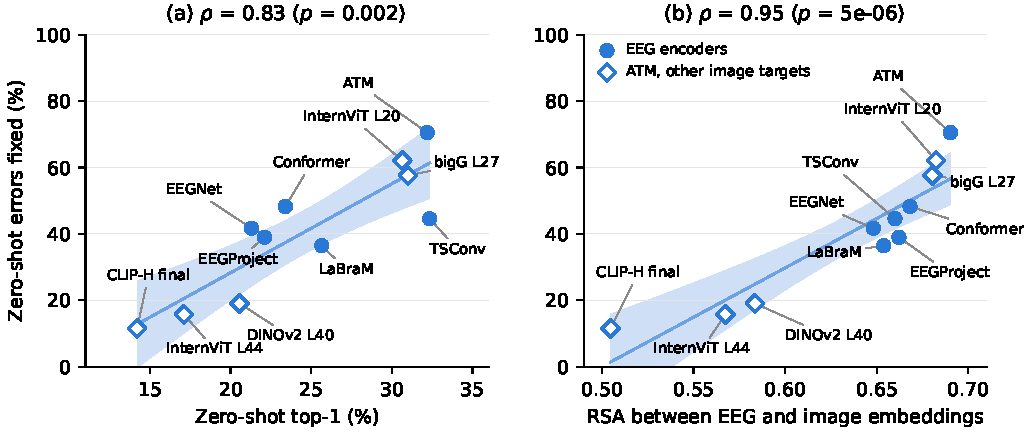
\includegraphics[width=\textwidth]{figures/encoders.pdf}
  \caption{Calibration gain across encoders and image targets. Fraction of the zero-shot errors fixed by GALA against (a) the zero-shot top-1 accuracy and (b) the RSA between EEG and image embeddings, for the six encoders of Table~\ref{tab:encoders} (filled circles) and for ATM trained against five other image targets (open diamonds). Lines: least-squares fit over the 11 models with its 95\% confidence band. $\rho$: Spearman's correlation over the 11 models.}
  \label{fig:encoders}
\end{figure*}

To assess the robustness of our framework, we evaluate GALA across EEG encoder architectures (Table~\ref{tab:encoders}, Fig.~\ref{fig:encoders}). GALA fixes 38\% to 73\% of the zero-shot errors of the six encoders, but zero-shot accuracy does not predict this fraction ($\rho=0.20$, $p=0.70$; Fig.~\ref{fig:encoders}a): for instance, ATM and TSConv have roughly the same zero-shot accuracy, but GALA fixes 73\% of the errors of ATM and 46\% of those of TSConv. We also measure the representational similarity (RSA)~\cite{kriegeskorte2008rsa} between the two modalities, as the correlation between the pairwise cosine similarities of the centered test EEG embeddings and those of their images. It is invariant to rotations of either space: two clouds with identical similarity matrices are related by an orthogonal map. Therefore, RSA measures how close the EEG cloud is to a rotated copy of the image cloud, which is precisely the relation GALA's rotation exploits. Over the six encoders, ATM has the highest RSA and the largest gain, but the RSA of the five other encoders spans only 0.02, and the correlation is not significant ($\rho=0.49$, $p=0.33$). To widen this range, we train ATM against five other image targets: intermediate layers of InternViT-6B (layer 20) and OpenCLIP bigG~\cite{cherti2023openclip} (layer 27), and the final or near-final layers of CLIP ViT-H~\cite{radford2021clip}, InternViT-6B (layer 44) and DINOv2~\cite{oquab2024dinov2} (layer 40). The final layers lower both the RSA (0.50 to 0.58) and the fraction of errors fixed (14\% to 19\%). Over the 11 models, RSA predicts the gain ($\rho=0.92$, $p<10^{-4}$; Fig.~\ref{fig:encoders}b) better than zero-shot accuracy ($\rho=0.78$; Fig.~\ref{fig:encoders}a), and remains correlated with it at fixed zero-shot accuracy (partial $\rho=0.78$, against $0.17$ for zero-shot accuracy at fixed RSA).

\begin{figure*}[t]
  \centering
  \includegraphics[width=\textwidth]{figures/regimes.pdf}
  \caption{Streaming and open-gallery results (ATM, 10 subjects). (a) Streaming (R2): top-1 on the buffer at each of the 50 refits, averaged over menus, repetitions and stream orders. (b) Open gallery (R3): $D$ distractor images are added to the 200 candidates.}
  \label{fig:regimes}
\end{figure*}

\subsection{Streaming (R2)}
\label{sec:stream}

In R2, queries are drawn from a random menu of $K \in \{25, 50, 100, 150, 200\}$ images, averaged over $q \in \{5, 10, 20, 40\}$ repetitions, and arrive in random order. The calibration is re-fitted 50 times along the stream, and all trials received so far are decoded with the latest fit. While GALA is harmful at the start of the stream, damping makes it beneficial regardless of the size of the buffer. 

\subsection{Open Galleries (R3)}
\label{sec:regimes}

In R3, $D$ distractor images that are never queried are added to the 200 candidates. GALA approaches the zero-shot decoder as $D$ grows and falls to its level at $D=1{,}654$ (11.3\% vs 11.5\%; Fig.~\ref{fig:regimes}b). This failure comes from the balanced transport, which assigns mass to images that are never queried: when GALA is restricted to the images actually present, it recovers its R1 accuracy at every $D$.

\subsection{Comparison with Supervised Alignment}
\label{sec:labels}

% numbers of this subsection: ATM ValCon, three seeds
\paragraph{Number of labels.}
We fit a supervised orthogonal map on $n$ labeled pairs from the training session of the target subject, on concepts disjoint from the test set, and score it with CSLS like GALA. Even with all 16{,}540 labeled pairs of the session, the supervised map (80.3\%) stays below GALA fitted on the 200 unlabeled test queries (81.8\%). The two are complementary: applying GALA after the supervised map gives 91.5\%.



%=====================================================================
\section{Discussion and Conclusion}
\label{sec:discussion}

\paragraph{Evaluation benchmarks and community standards.}
Much of this literature~\cite{zhang2025neurobridge,du2025shallow,huang2026sattc} selects the checkpoint on the held-out subject, since THINGS-EEG-2 does not natively offer a validation set. This is a form of information leakage: on ATM, we measured that it inflates zero-shot accuracy by 3.6 points compared to our validation-selected checkpoints. We encourage future work in this area to adopt a validation split, such as the held-out training concepts we use, as the primary reported metric. Moreover, the standard 200-way test set from THINGS-EEG-2 presents a bijective structure between the two modalities, that can be leveraged and optimized for, despite not being representative of real-life BCI deployment conditions. We encourage future work to report the Hungarian assignment as a control for this particular setup, to report the number of averaged repetitions, per-subject results, and to provide other regimes beyond the bijection. More broadly, the field would strongly benefit from the development of additional visual decoding benchmarks. Most previous studies have evaluated their methods exclusively on THINGS-EEG-2, which raises concerns about dataset-specific conclusions. \TODO{Alljoined-1.6M and THINGS-MEG results.} 

\paragraph{Limitations and future work.}
GALA relies partially on the availability and presence of the candidate gallery, and degrades when distractors are added. Deciding without labels which candidates are present remains an open problem. More broadly, our evaluation, like the benchmark it builds on, replays offline recordings of a rapid serial visual presentation paradigm, in which each query averages many repetitions of the same image. A deployed BCI rarely offers these conditions: the candidate set changes with the task of the user, queries arrive one at a time and from few repetitions, and calibration must happen online. Evaluations that reproduce these conditions, with task-dependent candidate sets, closed-loop sessions and single-trial queries, would measure more realistically what transductive calibration brings in practice. 

\paragraph{Conclusion.}
We argue for gallery-level alignment as a way to deploy EEG decoders on new users without labeled calibration data, formalize the label-free transductive setting, the assumptions under which it should be evaluated, and introduce GALA. On the standard test setup of THINGS-EEG-2, GALA brings the top-1 accuracy from 32.2\% to 81.8\%. We hope that these contributions will help put forward transductive test-time calibration as a more realistic and practical alternative to the current benchmarking methods within the broader context of BCI deployment.

\section*{LLM Usage Statement}
Claude (Anthropic) was used as a coding agent and an aid in the redaction of the article. It wrote and ran part of the experiments, produced the figures, and drafted and edited parts of the text. All of his outputs have been extensively verified by the authors. 

{
    \small
    \bibliographystyle{ieeenat_fullname}
    \bibliography{references}
}

\clearpage
\appendix
\section{Streaming Results per Menu Size and Number of Repetitions}
\label{app:stream}

\begin{figure*}[t] 
  \centering
  \includegraphics[width=\textwidth]{figures/stream_grid.pdf}
  \caption{Streaming (R2) results for each menu size $K$ (columns) and number of averaged repetitions $q$ (rows), ATM, 10 subjects, three training seeds and three stream orders. The x-axis is the total stimulus time needed to collect the buffer, at 200\,ms per repetition (100\,ms image and 100\,ms blank).}
  \label{fig:streamgrid}
\end{figure*}

Figure~\ref{fig:streamgrid} details the streaming results of Fig.~\ref{fig:regimes}a for each menu size $K$ and number of averaged repetitions $q$. Every stream eventually contains all 80 repetitions of each menu image, so for a given $K$ the streams end after the same stimulus time for every $q$. Without damping, the drop of GALA at the first refit grows with $q$, from 11 points at $q=5$ to 37 points at $q=40$, since the buffer then holds fewer queries. With damping, GALA is never more than 3 points below the zero-shot decoder, at any refit of any configuration.

\end{document}
